\section{Approach}\label{sec:approach}

After discussing the boot reliability problem with the IlliniSat team, we decided to develop a fault model that realistically represented the threat of cosmic ray related failures in space.  We chose to model the system as two component subsystems: the storage (or Flash) subsystem and the execution (or RAM) subsystem.  A failure in the Flash subsystem indicates that the Flash memory that contains the operating system kernel is no longer correct or that the Flash memory is unable to correctly respond to read or write requests.  A failure in the RAM subsystem indicates that the operating system has encountered a fatal error and must be rebooted by the watchdog timer.  The system has failed when both subsystems have failed simultaneously; the failure of the RAM subsystem causes the system to reboot, while the failure of the Flash subsystem means that no valid operating system kernels exist to boot.  Note that we do not consider application-level crashes or failures in this model.

Our literature review revealed the following failure modes for each of the systems.

\subsubsection{Flash System}\label{sec:flashmodel}
\begin{itemize}
  \item {\bf Single Event Upset (SEU):} This failure mode occurs when a cosmic ray strikes a single bit in a memory, causing it to change \cite{Gerardin2010Present}.  SEUs are part of a class of faults called Single Event Effects (SEEs).  SEE testing has been standardized \cite{Schwank2013Radiation} and many experimental studies have measured the SEU error rate for different devices \cite{Langley2004SEE, Oldham2008TID}.
  \item {\bf Single Event Latchup (SEL):} This failure mode causes a high operating current in the device that could eventually permanently damage the chip.  One study that measures SEL resistance in a chip is \cite{Langley2004SEE}.
  \item {\bf Single Event Functional Interrupt (SEFI):} This failure mode occurs when the memory's control circuitry is struck by a cosmic ray, causing it to transition to an undefined state \cite{Langley2004SEE}.  SEFIs may generally be repaired by either attempting to repeat the desired operation or by power-cycling the controller to place it into a known state \cite{Gerardin2010Present}.
  \item {\bf Total Ionizing Dose (TID):} As cosmic rays strike a device over time, the device may degrade, causing reduced performance or failure \cite{Gerardin2010Present}.  TID testing has also been performed in the laboratory for various devices \cite{Oldham2008TID}.
\end{itemize}
\subsubsection{RAM System}\label{sec:rammodel}
\begin{itemize}
\item
\end{itemize}

Among these failure modes, we chose to model SEU and SEFI failures for the Flash system and SEU, multiple-bit, and device failures for the RAM system.  We chose to intentionally omit SELs from the Flash model because they only appear to be activated at higher ion energies; one example 1GB flash memory experienced SEL effects between 43 and 53 MeV $\cdot$ cm$^2$/mg \cite{Langley2004SEE}, which indicates that latchup is unlikely to occur \cite{Schwank2013Radiation}.  Similarly, TID testing often reveals that the necessary dose to cause failure in a chip is greater than 50kRad \cite{Oldman2008TID}, which is over double the dose that a CubeSat's C\&DH board is likely to experience over a 1-year mission \cite{Likar2010Novel}.  While multiple-bit errors could occur in the flash system, we assume that their absence in papers discussing SEE effects indicates that they are not a major concern for nonvolatile memory.

\subsection{Developing a Fault Model}\label{sec:developingmodel}



\subsection{Building the Fault Model in M\"obius}\label{sec:buildingmodel}

We chose to motivate the development of the boot protection script by developing a SAN model in M\"obius.

We choose to measure reliability as the relevant dependability metric because the continuous operation of the satellite is critical to the IlliniSat team; furthermore, the failure that we are modeling is catastrophic.  As the satellite cannot recover from any failure of this type, it does not make sense to measure the system's availability.

The parameters used in this model are shown in Table \ref{tab:parameters}.

\begin{table}[width = 0.5\textwidth]
\centering
\begin{tabular}{|c|c|c|c|}
\hline
{\bf Parameter Name} & {\bf Description} & {\bf Value} & {\bf Source}\\
\hline
\texttt{seu\_rate} & SEU event rate & & \\
\hline
\end{tabular}
\caption{Parameters used in the M\"obius model}
\label{tab:parameters}
\end{table}
\subsection{Boot Protection}
The C\&DH system uses a Linux kernel that is booted by
U-boot.\footnote{\url{http://www.denx.de/wiki/U-Boot}} The fault model
considered here is bit corruption in the Linux kernel that is present at boot
time.  Currently, there is only one copy of the Linux kernel and if it fails to
boot, the entire C\&DH system will experience catastrophic failure.  The
solution described below is designed to reduce that single point of failure to a
much smaller region of code.  When considering the reliability of U-boot itself,
the C\&DH board already uses the MLO bootloader with redundant U-Boot images.

\subsubsection{Test Environment}
In order to develop and test the boot protection system in a controlled
environment, we decided to use an ARM emulator.  The QEMU~\cite{bellard2005qemu}
emulator is well known and supports a variety of architectures, including
several ARM development boards.  It does not currently support the MityARM board
used by IlliniSat, so we use the ``versatilepb'' virtual development board to
run U-boot and Linux compiled for
ARM.\footnote{\url{http://elinux.org/Virtual_Development_Board}}

The initial bulk of this work involved getting the test environment running and
we have made detailed notes so that we can share this procedure with others
working on similar problems.  The versatilepb board in QEMU has a virtual flash
drive that is memory mapped to address 0x3400000, which we use to store the
contents of the OS kernel images and the boot protection scheme.

\subsubsection{Implementation}
U-Boot has built-in support for CRC-32, and every image (e.g. application, OS,
script, filesystem, etc...) is stored in a format that contains this checksum.
Therefore, one can use this built-in functionality to validate checksums.
U-Boot can be configured with a script interpreter that will run pre-complied
scripts that are very similar to typical Unix shell scripts. Using this
functionality, we developed a script that will check kernel images before
booting. The script iterates through multiple kernel images until it finds one
with a valid CRC checksum and boots that one.  If no valid checksums are found,
it will attempt to boot the first image.  

Figure \ref{fig:mem_map} shows the memory map of the boot protection scheme
used in the QEMU test environment.  In this case, the script is 914B and each
kernel image is 1.7MB.  Without this scheme, the Linux kernel image was a
single-point-of-failure during the boot process (or one could boot a faulty
kernel and have other failures at a later time).  The script effectively reduces
the area vulnerable to bit errors by three orders of magnitude (1.7MB/914B =
1950).  It is important to note that since the QEMU development environment used
a memory-mapped flash device, the kernels are shown as being contiguous in
memory.  However, it would be trivial to modify the script to load the kernels
from a separate device (e.g. an SD card, as found on the MityARM335x).

%(1.7 megabytes) / (914 bytes) = 1950.30547

%Include: SD card and memory map stuff
\begin{figure}
  \centering
  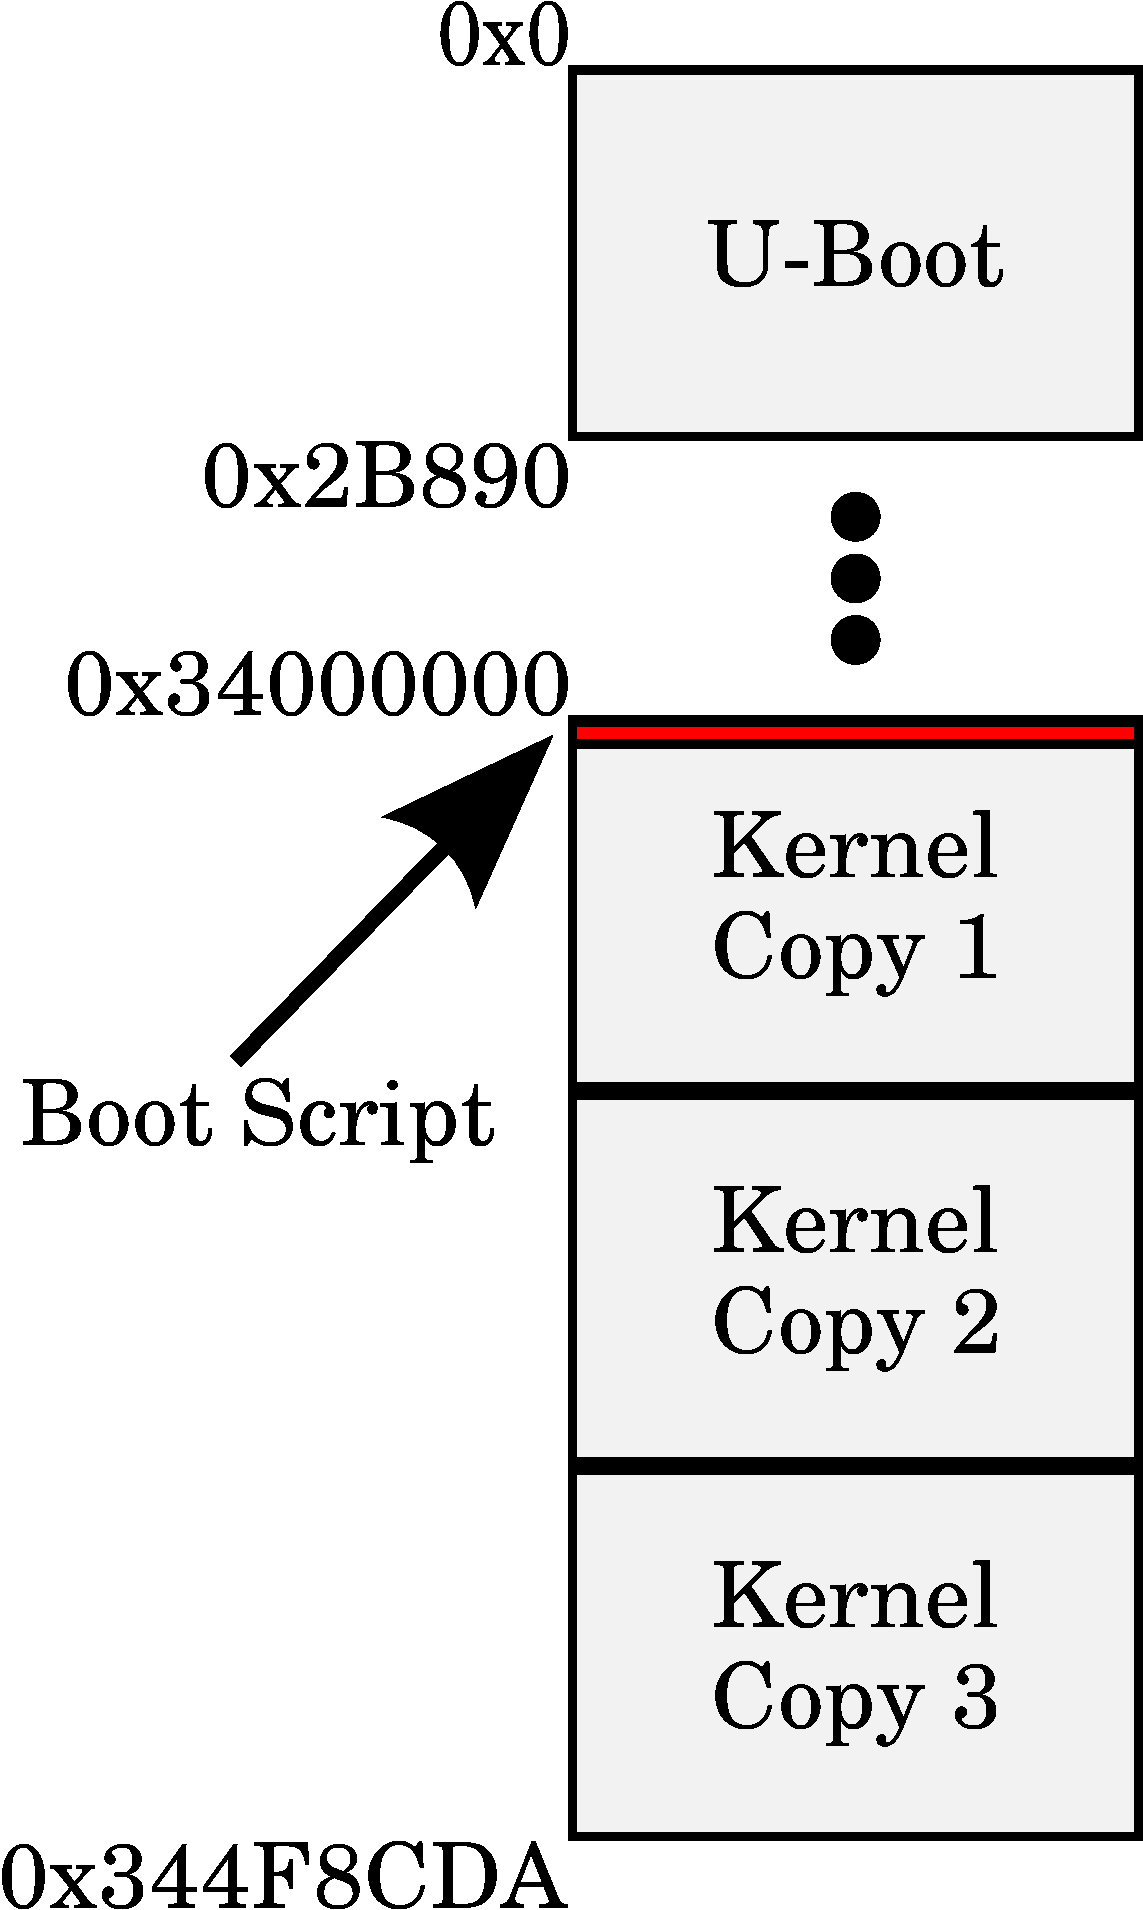
\includegraphics[width=0.15\textwidth]{images/mem_map}
  \caption{The memory map used to evaluate the boot protection system in QEMU.
           The U-boot application itself occupies 0.17MB, whereas the protection
           script is 914 bytes and each Linux kernel is
           1.7MB.}\label{fig:mem_map}
\end{figure}

%END BOOT - MERGE ANCHOR
\subsection{Flash Patrol Daemon}
The flash patrol daemon watches the filesystem that is on the device's flash memory and 
generates CRCs on each creation or modification of a file. The daemon uses the linux 
inotify\footnote{\url{http://man7.org/linux/man-pages/man7/inotify.7.html}} API 
to monitor any and all events to individual files or within selected directories 
using a series of system calls. Inotify is accessed using a file descriptor (fd)
that is passed back from the inotify initialization function. Using this fd, we are able to add files 
and directories into the inotify ``watch list.'' The events can then be accessed 
by reading the inotify fd. However, since this mission calls for low power 
consumption, a naive polling implementation would not be ideal.

Instead, we have used the select() function to implement a signal-based approach. This function
will only return once it has received a signal that indicates that the inotify fd has been used.
Once the select function returns, we know that there is an event that we need to process. We iterate
through all of the events that we get from the read of the inotify fd and process them all separately.
For all file creations and modifications in the currently watched directory, we generate a 32-bit CRC 
for the created/modified file and then store this CRC in a new file. By using CRC-32 we are
able to detect all 1-bit errors and burst errors that are equal to or less than 32 bits apart. This checksum is
relatively simple, but still gives us decent error detection. Since we are conscious about the amount
of time we spend on computations, CRC-32 fits perfectly. 

\subsection{CRC Checker Daemon}
The CRC checker daemon is the complement daemon to the flash patrol daemon. The flash
patrol daemon watches the filesystem and generates CRCs, while the CRC checker periodically
parses the directories that inotify is watching and checks the generated CRCs. The daemon will 
sleep for a predefined amount of time and then parse the watched directories. To check the CRCs
the daemon will recompute the CRC for each one of the files and then check that CRC against the
one that was generated earlier by the flash patrol daemon. The two daemons use the exact same
CRC-32 generation function, so the daemon will be able to detect errors that occur in the 
files. 














